% Preamble ==================================================================
\documentclass[11pt]{article}
\usepackage{geometry}
\geometry{verbose,tmargin=2.5cm,bottom= 1.5cm,lmargin=2.5cm,rmargin=2.5cm}
\usepackage{float}
\usepackage{graphicx}
\usepackage{amsmath}
\usepackage{amssymb}
\usepackage{enumitem}
\usepackage{mathtools}

\usepackage{amsthm} % theorem
\usepackage{listings} % code snippets
\usepackage{fancyvrb} %verbatim
\usepackage{xcolor}  % color math
\lstset{frame=l,
  language=Python,
  basicstyle={\small\ttfamily},
  numbers=none,
  numberstyle=\tiny\color{black},
  keywordstyle=\color{black},
  commentstyle=\color{blue},
  stringstyle=\color{mauve},
}

\numberwithin{equation}{section}

\usepackage{titlesec,dsfont}

%Format section heading style
\usepackage{sectsty}
\sectionfont{\sffamily\bfseries\large}
\subsectionfont{\sffamily\normalsize\slshape}
\subsubsectionfont{\sffamily\small\itshape}
\paragraphfont{\sffamily\small\textbf}


%Put period after section number
\makeatletter
\def\@seccntformat#1{\csname the#1\endcsname.\quad}
\makeatother

%Bibliography
\usepackage[round]{natbib}
\bibliographystyle{genetics}

%Format captions
\usepackage[ labelsep=period, justification=raggedright, margin=10pt,font={small},labelfont={small,normal,bf,sf}]{caption}

\setlength{\parskip}{0ex} %No space between paragraphs.

\renewcommand{\familydefault}{\sfdefault}

\newcommand\indep{\protect\mathpalette{\protect\independenT}{\perp}}
\newcommand{\nindep}{\not\!\perp\!\!\!\perp}
\def\independenT#1#2{\mathrel{\rlap{$#1#2$}\mkern2mu{#1#2}}}

%PUT ME LAST--------------------------------------------------
\usepackage[colorlinks=true
,urlcolor=blue
,anchorcolor=blue
,citecolor=blue
,filecolor=blue
,linkcolor=black
,menucolor=blue
,linktocpage=true
,pdfproducer=medialab
,pdfa=true
]{hyperref}

\makeatother %Put this last of all


\newcommand{\defeq}{\coloneqq}
\newcommand{\overbar}[1]{\mkern 1.5mu\overline{\mkern-1.5mu#1\mkern-1.5mu}\mkern 1.5mu}

% Make theorems bold
\makeatletter
\def\th@plain{%
  \thm@notefont{}% same as heading font
  \itshape % body font
}
\def\th@definition{%
  \thm@notefont{}% same as heading font
  \normalfont % body font
}
\makeatother

\newtheorem{thm}{Theorem}[section]
\newtheorem{defn}{Definition}[section]
\newtheorem{cor}{Corollary}[section]
\newtheorem{prop}{Property}[section]
\newtheorem{rle}{Rule}[section]
\newtheorem{lma}{Lemma}[section]

\definecolor{dred}{HTML}{c90404}
\definecolor{dgreen}{HTML}{0b8717}
\definecolor{dmagenta}{HTML}{c904c6}

%Preamble end--------------------------------------------------


\begin{document}

\begin{flushleft}
\textbf{\Large Geometric Deep Learning}
\end{flushleft}

\begin{flushleft}
Author: Juvid Aryaman

Last compiled: \today
\end{flushleft}

\noindent This document contains my personal notes on Geometric Deep Learning, largely based on \cite{Bronstein21}\footnote{See also \url{https://geometricdeeplearning.com/}}.

\section{High-dimensional learning}

We discuss the curse of dimensionality in supervised machine learning to motivate why inductive priors are helpful to construct. We'll consider the data domain to be $\mathbb{R}^d$ for this particular discussion.

\subsection{Notation}

\newcommand{\eloss}{\tilde{\mathcal{R}}}
\newcommand{\ploss}{\mathcal{R}}
\newcommand{\hypclass}{\mathcal{F}}

\begin{itemize}[noitemsep]
\item Data $\mathcal{D} = \{(x_i, y_i)\}_i$, drawn i.i.d.\ from an underlying data distribution $P$ over $\mathcal{X} \times \mathcal{Y}$.
\item Assume data generated by unknown function $y_i = f(x_i)$.
\item Assume $\mathcal{X} = \mathbb{R}^d$ and $\mathcal{Y} = \mathbb{R}$.
\item The model, or hypothesis class, is a subset $\hypclass \subset \{f: \mathcal{X} \rightarrow \mathbb{R} \}$.
\item The hypothesis class is assumed to come equipped with a complexity measure of all elements: $\gamma: \hypclass \rightarrow \mathbb{R}$. This can usually be defined as a norm, making $\mathcal{F}$ a \textbf{Banach space}.
\item The (convex) error metric $l(y, y')$, e.g. squared error $l(y,y')=|y-y'|^2$.
\item Loss. Consider $\tilde{f} \in \mathcal{F}$
	\begin{itemize}[noitemsep]
	\item Population loss: $\ploss(\tilde{f}) = \mathbb{E}_P[l(\tilde{f}(x), f(x))]$. This is the true loss of the hypothesis, averaged over the entire data domain.
	\item Empirical loss: $\eloss(\tilde{f}) = 1/n \sum_i l(\tilde{f}(x_i), f(x_i))$. This is the loss over some finite sample $\mathcal{D}$.
	\end{itemize}
\end{itemize}


\newcommand{\hypdelta}{\hat{f}}
\newcommand{\infimum}[1]{\underset{#1}{\text{inf}}}
\subsection{Empirical risk minimization}

The underlying goal in supervised learning is to minimise the population loss $\mathcal{R}(\tilde{f})$ given only access to the empirical loss. We seek to construct a bound for the population loss of a hypothesis. Consider $\hat{f} \in \hypclass_\delta$, where $\hypclass_\delta = \{f \in \hypclass; \gamma(f) < \delta\}$, i.e. a hypothesis with bounded complexity. We then decompose $R(\hypdelta)$ as follows:
\begin{align}
\color{dred}{\ploss(\hypdelta) - \infimum{f \in \hypclass} \ploss(f)} &= \textcolor{blue}{\left(\eloss(\hypdelta) - \infimum{f \in \hypclass_\delta} \right)} \textcolor{dgreen}{+ \left[\left(\ploss(\hypdelta) - \eloss(\hypdelta)\right) - \left( \infimum{f \in \hypclass_\delta} \ploss(f) - \infimum{f \in \hypclass_\delta} \eloss(f) \right) \right]} \nonumber \\
&\color{dmagenta}{+ \left( \infimum{f \in \hypclass_\delta} \ploss(f) - \infimum{f \in \hypclass} \ploss(f) \right)}
\end{align}
where
\begin{itemize}
\item The {\color{dred}{red}} term is the population loss of the hypothesis $\hypdelta$ relative to the best-possible hypothesis in the hypothesis class $\hypclass$.
\item The {\color{blue}{blue}} term is the {\color{blue}{optimization loss}}, i.e. how close the empirical loss of the hypothesis gets to the best possible hypothesis in the ball of hypotheses considered $\hypclass_\delta$. Call this $\epsilon_\text{opt}$.
\item The {\color{dgreen}{green}} term is the {\color{dgreen}{statistical error}}, denoting noise from the finite sample used to evaluate the empirical loss, relative to the sampling noise from the best hypothesis in the ball. This can be bounded from above by [\textbf{TODO: Didn't understand how}]
\begin{equation}
\epsilon_\text{stat} = 2\underset{f \in \hypclass_\delta}{\text{sup}} |\ploss(f) - \eloss(f)|
\end{equation}
\item The {\color{dmagenta}{magenta}} term is the {\color{dmagenta}{approximation error}}, denoting how close the constrained hypothesis class can get to the best function in the unconstrained hypothesis class. Call this $\epsilon_\text{approx}$.
\end{itemize}
Thus
\begin{equation}
\ploss(\hypdelta) \leq \infimum{f \in \hypclass} \ploss(f) + \epsilon_\text{opt} + \epsilon_\text{stat} + \epsilon_\text{approx}.
\end{equation}
If the hypothesis class is dense then the infimum term is 0, e.g. neural networks with non-polynomial activation (Universal Approximation Theorems). Generally, as the approximation error reduces (through a larger hypothesis space, increasing $\delta$), the statistical error increases. 

\subsection{Learning Lipschitz functions}
\begin{defn}[Lipschitz function]
A function $f: \mathcal{X} \subseteq \mathbb{R}^d \rightarrow \mathbb{R}$ is $\beta$-Lipschitz if 
\begin{equation}
|f(x)-f(x')| \leq \beta ||x-x'||
\end{equation}
i.e. the function cannot vary ``too quickly''. 
\end{defn}
If $f$ is 1-Lipschitz, and $P=\mathcal{N}(0, I_d)$, and using empirical risk minimization of the previous section, then a lower-bound on the amount of data required to estimate $f$ up to error $\epsilon$ grows as $\epsilon^{-d}$. The curse of dimensionality also crops up in e.g. using a single-layer perceptron to approximate a high-dimensional function, where the statistical error is cursed by dimension. 

However, in most cases, data are not simply points in a high-dimensional space: rather, the are \textbf{signals} on a low-dimensional \textbf{manifold} embedded in a high-dimensional input space $\mathcal{X}$ (Fig.~\ref{fig:geom-func-spaces}). The aim of an inductive prior (which is what Geometric Deep Learning is all about) is to reduce the size of the hypothesis space and thereby reduce statistical error, whilst also keeping the approximation error low, by limiting ourselves to hypothesis spaces which respect the symmetries of the data domain.

\begin{figure}
\begin{center}
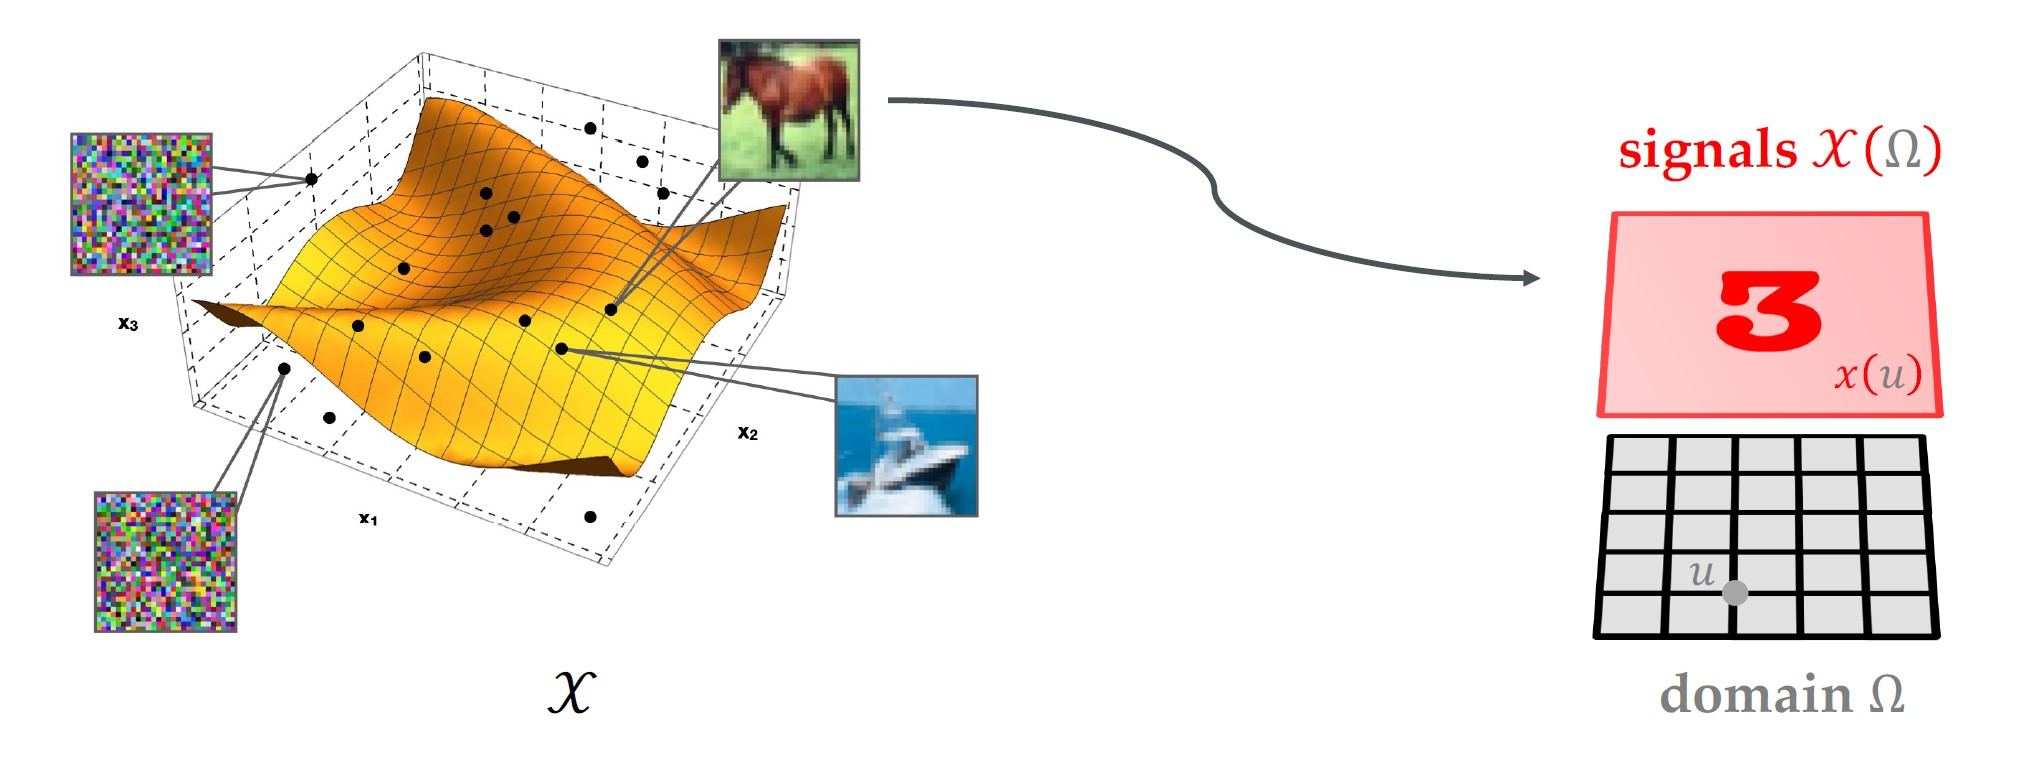
\includegraphics[width=0.8\columnwidth]{../figures/geometric-function-spaces.jpg}  
\end{center}
\caption{Geometric function spaces will allow us to exploit an underlying low-dimensional structure in the high-dimensional input space $\mathcal{X}$. For example, the space of all possible images are high-dimensional, but ``interesting'' images will exist on a lower-dimensional manifold embedded in the space of all images. Images off-manifold will look like boring noise. Geometric Deep Learning argues that data will often exist either on a grid, a graph, a group, or a manifold. Each of these have corresponding symmetries which can be leveraged.
}
\label{fig:geom-func-spaces}
\end{figure}

\newcommand{\f}{\mathfrak}
\section{Geometric priors}

\subsection{Preliminary definitions}
\begin{itemize}[noitemsep]
\item Assume that data ``lives'' on a domain $\Omega$. Domain is a \textbf{set}, possibly with additional structure
\item Data is a \textbf{signal} (function) on the domain $x : \Omega \rightarrow \mathcal{C}$
\item Dimensions of vector space $\mathcal{C}$ are \textbf{channels}
\item The space of $\mathcal{C}$-valued signals is $\mathcal{X}$, where $\mathcal{X}(\Omega, \mathcal{C}) = \{x: \Omega \rightarrow \mathcal{C} \}$
\end{itemize}

For example, an $n \times n$ RGB image can be considered a function which maps an element of the domain $\Omega = \mathbb{Z}_n \times \mathbb{Z}_n$ onto an element of the vector space $\mathcal{C}=\mathbb{R}^3$. 

\begin{defn}[Addition and scalar multiplication on signals] \label{defn:add-mul-signals}
Let $x,y \in \mathcal{X}$. Define addition and scalar multiplication of signals through pointwise multiplication over the domain: 
\begin{equation}
(\alpha x + \beta y)(u) = \alpha x(u) + \beta y(u)
\end{equation}
for all $u \in \Omega$ with scalars $\alpha, \beta \in \mathbb{R}$.
\end{defn}

\begin{thm}[Space of signals is a Hilbert space]
Assuming that $\mathcal{C}$ has an inner product $\langle v, w \rangle_\mathcal{C}$, and there exists a measure $\mu$ on $\Omega$, we can define an inner product on $\mathcal{X}(\Omega, \mathcal{C})$ as
\begin{equation}
\langle x, y \rangle = \int_\Omega \langle x(u), y(u) \rangle_\mathcal{C}\ \mathrm{d}\mu(u). \label{eq:inner-prod-signals}
\end{equation}
Given this inner product, and the fact that Defn.~\ref{defn:add-mul-signals} implies that $\mathcal{X}$ is a vector space, then the space of signals $\mathcal{X}$ is therefore a Hilbert space.
\end{thm}

If $\Omega$ is a finite set then $\mu$ can be chosen as the counting measure and the integral in Eq.\eqref{eq:inner-prod-signals} becomes a sum. The existence of an inner product allows us to perform ``pattern matching'', for example comparing a signal $x$ to a filter $y$. There can be cases where the domain itself are the data: e,g. meshes, or graphs without node or edge features. But we can often turn the domain into a signal on the domain itself, e.g. the adjacency matrix $A_{ij}$ is a signal on $\Omega \times \Omega$.

Note that, in the most general case, data are maps from a point in the domain to a vector space \textbf{indexed} by the point in the data domain: $x: \Omega \rightarrow \mathcal{C}_u$. For example, the tangent space for a point $u$ on a spherical manifold $\Omega$ varies for every point $u$. In this case, the data aren't functions but \textbf{fields} (or \textbf{sections of a bundle}), and the space $\mathcal{C}_u$ is called a \textbf{fiber}. For simplicity we'll only work with function spaces $\mathcal{X}(\Omega, \mathcal{C})$ for now.

\begin{defn}[Group]
A \textbf{group}\footnote{Disturbingly, the authors choose to use Fraktur font to denote group elements, rather than Lie algebras which is more customary.} is a set $\mathfrak{G}$ along with a binary composition operation $\circ: \f{G} \times \f{G} \rightarrow \f{G}$ (for brevity, denoted as $\f{g} \circ \f{h} = \f{g}\f{h}$) satisfying:
\begin{itemize}[noitemsep]
\item Associativity: $(\f{gh})\f{l} = \f{g}(\f{hl})$ for all $\f{g}, \f{h}, \f{l} \in \f{G}$
\item Identity: there exists a unique $\f{e} \in \f{G}$ satisfying $\f{eg} = \f{ge} = \f{g}$ for all $\f{g} \in \f{G}$
\item Inverse: for each $\f{g} \in \f{G}$ there exists a unique inverse $\f{g}^{-1} \in \f{G}$ such that $\f{g g^{-1}} = \f{g^{-1}g} = \f{e}$
\item Closure: The group is closed under composition, i.e. for every $\f{g}, \f{h} \in \f{G}$ we have $\f{gh} \in \f{G}$
\end{itemize}
\end{defn}

\begin{defn}[Left group action]
If $\f{G}$ is a group with identity element $\f{e}$, and $X$ is a set, then a (left) group action $\alpha$ of $\f{G}$ on $X$ is a function
\begin{equation}
\alpha : \f{G} \times X \rightarrow X
\end{equation}
that satisfies the following two axioms:
\begin{enumerate}[noitemsep]
\item Identity: $\alpha(\f{e}, x) = x$
\item Compatibility: $\alpha(\f{g}, \alpha(\f{h}, x)) = \alpha(\f{gh}, x)$
\end{enumerate}
for all $\f{g}$ and $\f{h}$ in $\f{G}$ and all $x$ in $X$. We often shorten $\alpha(\f{g}, x)$ to $\f{g}x$ or $\f{g}\cdot x$ when the action being considered is clear from context.
\end{defn}


\begin{defn}[Abelian group]
An Abelian group is a particular type of group for which all elements commute, i.e. $\f{gh} = \f{hg}$ for all $\f{g},\f{h} \in \f{G}$.
\end{defn}

Importantly, the set of \textbf{symmetries} of an object form a group: these are the set of transformations which leave an object invariant.

\begin{defn}[Generating set of a group]
A generating set of a group is a subset of the group set such that every element of the group can be expressed as a combination of finitely many elements of the subset and their inverses.
\end{defn}

For example, the symmetry group of an equilateral triangle (dihedral group $D_3$) is generated by a $60^{\circ}$ rotation and a reflection. In contrast, the 1D translation group, is generated by infinitesimal displacements -- which is an example of a \textbf{Lie group} of differentiable symmetries. Note that, in specifying a symmetry group, we need only specify how the group elements \textbf{compose}, as opposed to what they \textit{are}. Hence, the same symmetry group can describe very different objects: for example the symmetry group of an equilateral triangle $D_3$ is the same as the groups of permutations on a sequence of three elements $\Sigma_3$.

\subsection{Group actions and representations on signals}
For a symmetry group $\f{G}$ operating on the space of signals $\mathcal{X}(\Omega)$, we can express a group action as satisfying
\begin{equation}
(\f{g}\cdot x)(u) = x(\f{g}^{-1}u) \label{eq:group-action-on-signal}
\end{equation}
see Fig.~\ref{fig:linearity-group-action} for a pictorial depiction of this\footnote{The inverse is required to obtain a valid group action that is associative, satisfying $(\f{g}\cdot(\f{h}\cdot x))(u) = ((\f{gh})\cdot x)(u)$. [\textbf{TODO:} Didn't understand why this wouldn't work without the inverse]}. Consider $x$ as an image, and $\f{g}$ to be a finite translation: e.g. a translation to the right. Then $(\f{g}x)(u)$, i.e. the translated image evaluated at some point $u$ in the domain, is the same as using the original image function, but translating the domain to the left. A consequence of Eq.\eqref{eq:group-action-on-signal} is that group actions on signals is \textbf{linear}, in the sense that
\begin{equation}
\f{g}\cdot(\alpha x + \beta x') = \alpha (\f{g}\cdot x) + \beta(\f{g} \cdot x')
\end{equation}
for real scalars $\alpha, \beta$ and signals $x, x' \in \mathcal{X}$. This linearity means that there exists a \textbf{representation} of such groups on signals:
\begin{defn}[Group representation]
A representation of a group $\f{G}$ on a vector space $V$ over a field $K$ is a group homomorphism from $\f{G}$ to the general linear group $GL(V)$
\begin{equation}
\rho: \f{G} \rightarrow GL(V)
\end{equation}
such that 
\begin{equation}
\rho(\f{g}_1 \f{g}_2) = \rho(\f{g}_1) \rho(\f{g}_2)
\end{equation}
for all $\f{g}_1, \f{g}_2 \in \f{G}$. In the case where $V$ has a finite dimension $n$, it is common to choose a basis for $V$ and identify $GL(V)$ with $GL(n, K)$, the group of $n \times n$ invertible matrices on the field $K$.
\end{defn}
Note that the particular form of the representation (and how it operates on elements of the vector space) will depend upon the dimensionality of the vector space it is acting on, even when considering the very same underlying group. In practice, even when the vector space $\Omega$ is infinite, one must always computationally discretize to find a finite grid, and therefore a finite-dimensional representation exists. I.e. we can find a map $\rho : \f{G} \rightarrow \mathbb{C}^{n \times n}$ that assigns a each group element $\f{g}$ an invertible matrix $\rho(\f{g})$. A representation is called \textbf{unitary} or \textbf{orthogonal} when the matrix $\rho(\f{g})$ is unitary or orthogonal for all $\f{g} \in \f{G}$.

\begin{figure}
\begin{center}
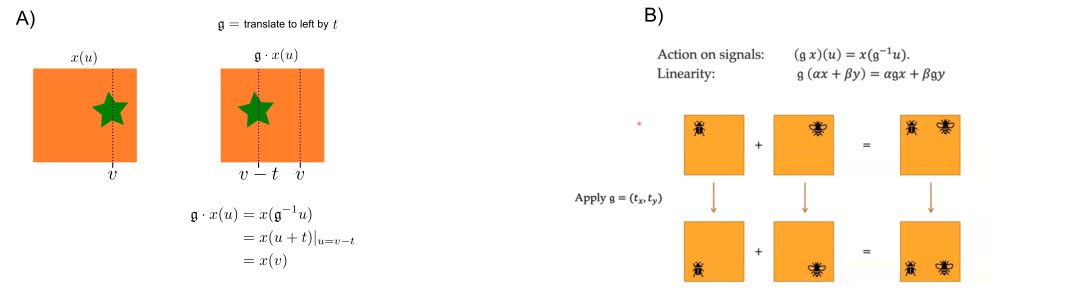
\includegraphics[width=\columnwidth]{../figures/group-action-linearity.png}  
\end{center}
\caption{Group action is linear on the space of signals. A) Consider a binary image $x$, a point on the underlying 2D grid $u$, and a symmetry group element such as a translation of the image to the left by $t$ pixels. Eq.\eqref{eq:group-action-on-signal} shows the effect of the group action on the image, which is to act inversely on the image domain: i.e. the image grid slides to the right by $t$ pixels and the same image is placed at that location. B) Linearity on signals means that if we add two signals, and then apply a symmetry transformation, that is the same as applying the symmetry transformation on each signal separately and then adding the result together. 
}
\label{fig:linearity-group-action}
\end{figure}

\subsection{Invariant and equivariant functions}
The symmetry of the domain $\Omega$ underlying signals $\mathcal{X}(\Omega)$ imposes structure on the function mapping the signal to the target $\mathcal{Y}$. Two important cases are invariant and equivariant functions.

\begin{defn}[Invariant function]
A function $f: \mathcal{X}(\Omega) \rightarrow \mathcal{Y}$ is $\f{G}$-invariant if 
\begin{equation}
f(\rho(\f{g})x)=f(x) \label{eq:inuivariant-fcn}
\end{equation}
for all $\f{g} \in \f{G}$ and $x \in \mathcal{X}(\Omega)$. I.e. its output is unaffected by the group action on the input.
\end{defn}

An example of an invariant function might be in image classification, where an image contains a particular object (e.g.\ a dog or a cat), and the abstract function $f$ mapping the image onto the true label is invariant to the position of the object in the image. In such settings, we often implement a convolutional neural network as the model. However, CNNs are not shift-invariant, but shift-equivariant.

\begin{defn}[Equivariant function]
A function $f: \mathcal{X}(\Omega, \mathcal{C}) \rightarrow \mathcal{X}(\Omega', \mathcal{C}')$ is $\f{G}$-equivariant if 
\begin{equation}
f(\rho(\f{g})x) = \rho'(\f{g})f(x) \label{eq:equivariant-fcn}
\end{equation}
for all $\f{g} \in \f{G}$. I.e. group action on the input affects the output in the same way, albeit with the possibility of the input and output spaces having different domains.
\end{defn}

A prototypical example of shift-equivariance is image segmentation: a segment mask must follow shifts in the input image. In deep learning, it is often not a good idea to build an invariant representation ``too soon''. In order to recognise an object, a model must first recognize its parts -- this is why neural networks should be deep. If representations of parts are invariant, then information about the \textit{relative pose} of parts is lost, see Fig.~\ref{fig:invariance-equivariance}A. Hence we want equivariant, not invariant, layers for the early parts of the network.

\begin{figure}
\begin{center}
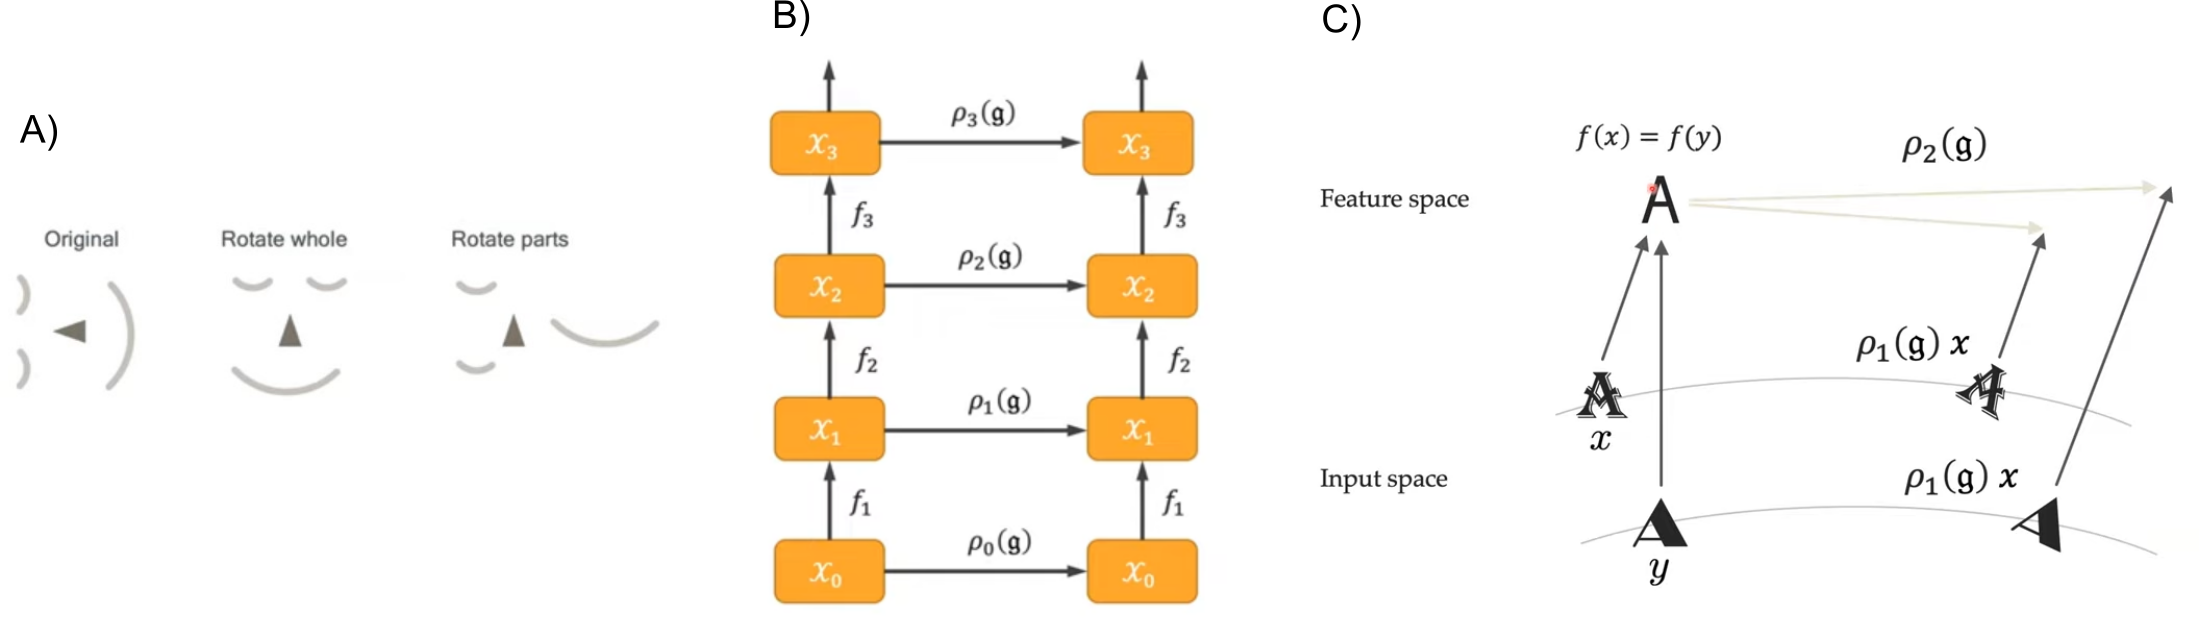
\includegraphics[width=\columnwidth]{../figures/invariance-equivariance.png}  
\end{center}
\caption{Equivariant layers are necessary in the early part of a neural network. A) In order for a neural network to recognise a face, it must first build representations of each of the parts: eyes, ears, mouth, nose. If the entire face is rotation invariant, that does not mean that each of the parts should be represented as rotation invariant, otherwise the relative orientation between the parts can be lost. B) On the left we have a sequential neural network, with layers $f_i$ and corresponding input signals $\mathcal{X}_{i-1}$. The arrows from left-to-right denote a symmetry transformation on the feature space. The image says that applying the symmetry transformation on the input (e.g. $\mathcal{X}_0$) and then applying the layer (e.g. $f_1$), should be the same as applying the layer and then applying the same symmetry transformation on the output(albeit on a different representation, e.g. $\mathcal{X}_1$). In other words, each layer obeys Eq.\eqref{eq:equivariant-fcn}. I.e. $f_i \circ \rho_{i-1}(\f{g}) = \rho_i(\f{g}) \circ f_i$ for each layer $i$. C) In practice, many neural network architectures will not generalize consistently across \textbf{orbits} of input. In this example of a CNN, rotating the input image will not result in a rotated representation but rather send the input space to different places in the feature space, because CNNs are not generally rotation equivariant.
}
\label{fig:invariance-equivariance}
\end{figure}

\newpage
\bibliography{geometric-dl.bib} 

\end{document}